\begin{figure}
  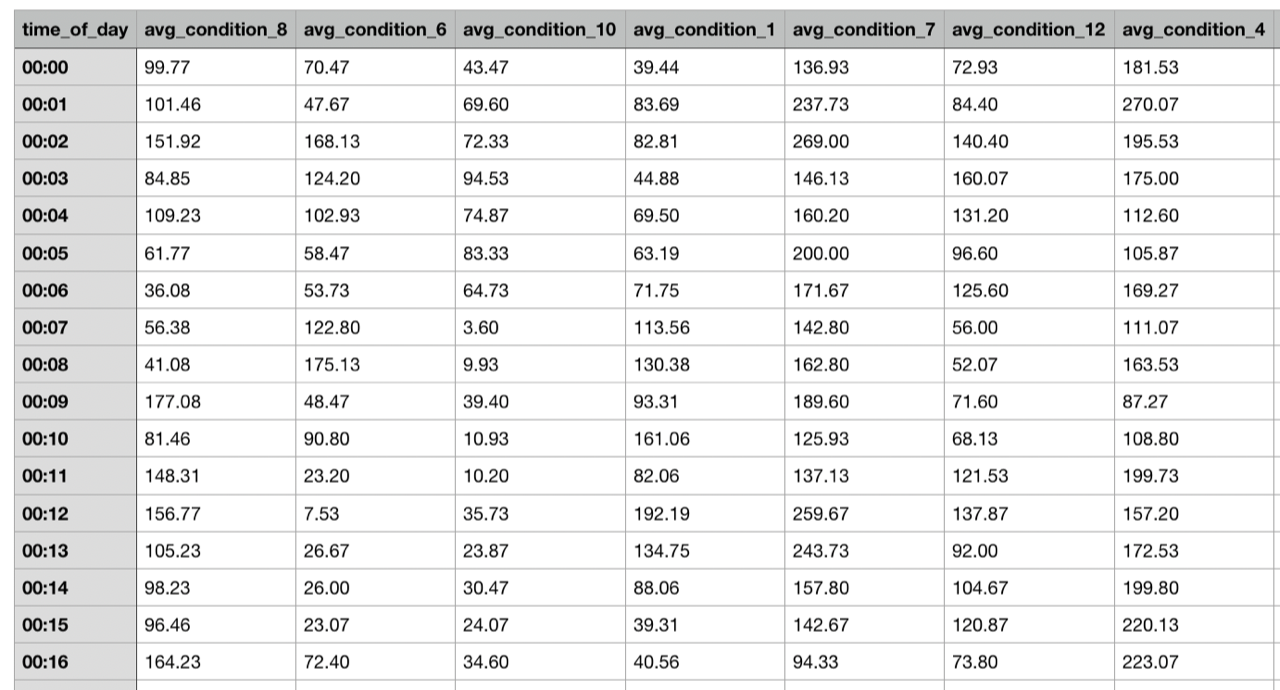
\includegraphics[height=7cm]{img/mean_by_tod.png}
  \caption{Dataset structured on mean activity level}
  \label{figure:mean_tod}
\end{figure}

To predict which group a given person belongs to, I need a good classification model. 
In order to predict something, we need some label that tells us what is correct. In this case, the filename tells us whether the person is 
in the \textit{control group} or \textit{condition group}, as described in the previous part. 

Since the dataset contains activity levels every minute of the recorded days, and the number of days for one participant varied,
I was thinking it might be a good idea to calculate the \textit{mean} activity for the participant at each minute every day.
This means that I can have a one-dimentional array of recordings for each participant instead of having an inconsistent number of rows. 

After structuring the dataset in this way, I ended up with one table where the Y-axis tells the minutes (from 00:00 to 23:59), 
and the X-axis contains all the participants. The data value at each position is then the mean activity for minute Y and participant X.
Table \ref{figure:mean_tod} is a small part of the dataset structured this way.

Now I just needed a classification model to handle this kind of data. After speaking with my supervisor about this, he mentioned 
Convolutional Neural Networks. 

I needed to learn more about CNNs. From what I knew from before, CNNs are used in image recognition. So I proceeded to implement image recognition.
Making it really simple, I wanted to classify images of cats and dogs. I went to one of my favorite websites for learning programming, https://pythonprogramming.net,
which is where I found a tutorial on 2D CNN for classification between images of cats and dogs \cite{2d_cnn}. 

It was both a fun and informative experience implementing this. Especially when I extended the script to allow an image url to predict on. 
Then I could browse for any image of a cat or a dog, and find out if the model could handle it (in most cases it did!). 
I even tried inputting images of humans to the model for fun. This experiment gave me a lot of motivation for my task.

\newpage

However, my data is one-dimentional, and image recognition is two-dimentional. The simple answer then is to use a 1D CNN.

\begin{quote}
  \textit{A 1D CNN is very effective when you expect to derive interesting features from shorter (fixed-length) segments of the overall data set 
  and where the location of the feature within the segment is not of high relevance. This applies well to the analysis of time sequences of sensor data 
  (such as gyroscope or accelerometer data).} \cite{1d_cnn}
\end{quote}

To learn more about 1D CNNs, I followed a tutorial \cite{1d_cnn}, which used a dataset containing 
time-sliced accelerometer data from a smartphone on the participants waists. The goal for this CNN is to predict what a given person is doing 
at the time, given the accelerometer data for that time slice. What the given person is doing is one of the following:
\begin{itemize}
  \item Standing
  \item Walking
  \item Jogging
  \item Sitting
  \item Upstairs
  \item Downstairs
\end{itemize}

As I followed the tutorial and implemented the model, I learned a lot about how 1D CNNs work, but also where my dataset could provide more data. 
What if the dataset contained the actual current state of the bipolar patient? Then we could make some automated system that always can tell a patient 
whether they are normal, manic or depressive! However data collection for this kind of task would be difficult because we can't always know what the
patient thinks, nor does the patient themselves. The "tutorial" dataset is different because it is easy to differientiate \textbf{physical} states of the body
like standing or walking.

